\documentclass[8pt]{beamer}
%epackage[french]{babel}
\usepackage[latin1]{inputenc}
\usepackage{listings}
\usepackage{times}
\usepackage{wasysym}
\usepackage[T1]{fontenc}


\definecolor{mongris}{gray}{0.8}           % definition couleur grise
\newcommand{\dd}{\footnotesize $\Diamond$}

\newcommand{\HH}{ \vspace{0.5pt}\hrule}
\newcommand{\round}[1]{\lceil #1 \rfloor}  % notation arrondi
\def\eme{$^{\textrm{{\`e}me}}$}                  % i {\`e}me
\def\num{n^{\circ}}                        % numero
\def\Num{N^{\circ}}                        % Numero
\def\sinc{\mathrm{sinc}}                   % sinus cardinal
\def\ere{$^{\textrm{{\`e}re}}$}                % {\`e}re
\def\er{$^{\textrm{{e}r}}$}                % {\`e}re
\def\eg{\emph{e.g.} }                      % e.g.
\def\ie{\emph{i.e.} }                      % i.e.
\def\etc{\emph{etc}}                       % etc
\def\cm{\,cm}                              % cm
\def\met{\,m}                              % m
\def\mm{\,mm}                              % mm
\def\deg{$^\circ$}                         % degres
\def\ud{\mathrm{d}}                        % pour dx dy ...


\def \R {{\Bbb R}}
\def \I {{\Bbb I}}
\def \H{{\Bbb H}}
\def \F {{\Bbb F}}
\def \S {{\Bbb S}}
\def \B {{\Bbb B}}
\def \Z {{\mathbb Z}}
\def \G {{\mathbb G}}
\def \L {{\mathcal{L}}}
\def \C {{\mathcal C}}
\def \P {{\mathcal P}}
\def \Q {{\mathcal Q}} 
\def \E{{\mathcal E}}
\def \D{{\mathcal D}}
\definecolor{mybluecolor}{RGB}{116,121,149}

\newcommand{\darky}[1]{{\usebeamercolor[fg]{block title example} #1}}
\newcommand{\myblue}[1]{{\color{mybluecolor}\aut{[#1]}}}

\newcommand{\ball}  {\ensuremath{B}}
\newcommand{\AMDR}{\operatorname{AMD}}
\newcommand{\AMD}{\operatorname{AMD}}

\newcommand{\MAset}{\ensuremath{\mathrm{A\!M}} }
\newcommand{\MAsetg}{\ensuremath{\MAset^g } }

\def \PS {{\aut{Planar-4-3-SAT}}}
\def \R {{\Bbb R}}
\def \I {{\Bbb I}}
\def \F {{\Bbb F}}
\def \S {{\Bbb S}}
\def \Z {{\mathbb Z}}
\def \L {{\mathcal{L}}}
\def \C {{\mathcal C}}
\def \P {{\mathcal P}}
\def \Q {{\mathcal Q}} 
\def \E{{\mathcal E}}
\def \D{{\mathcal D}}
\def \BD {{\bar{\mathcal{D}}}}
\def \etal {{\it et al.~}}
\def\arc{\mbox{arc}}
\definecolor{mongris}{gray}{0.8}          
\newcommand{\fup}[1]{\uparrow#1\uparrow}
\newcommand{\fdown}[1]{\downarrow#1\downarrow}
\newcommand{\sI}[1]{\overline{\tt #1}}
\newcommand{\iI}[1]{\underline{\tt #1}}
\newcommand{\e}[5]{#1 & #2 & #3 & #4 & #5 \\}
\newcommand{\eh}[5]{\text{#1} & \text{#2} &  \text{#3} &  \text{#4} & \text{#5}\\} 

\usepackage{beamerthemeliris2}
\useoutertheme{smoothbars}

\title[DGtal Meeting - Volumetric Package]{DGtal: Volumetric Geometry Package}
\subtitle{\url{http://liris.cnrs.fr/dgtal}}

\author{D. Coeurjolly}
%\author[DGtal~~~~~~~~~~~~~~~~~~~~~~~~~~David Coeurjolly]{David Coeurjolly}


 \newcommand{\fod}[2]{\multicolumn{2}{p{3.5cm}}{\emph{#1}\dotfill} &
      \multicolumn{2}{p{9cm}}{#2}\\}
    \newcommand{\fodt}[4]{\emph{#1} & {\footnotesize \textsl{#2}} & #3 & \small #4\\}
    % \newenvironment{ta}{\begin{tabular}{p{3.5cm}p{9cm}}}{\end{tabular}\\}
    \newenvironment{ta}{\begin{tabular}{crll}}{\end{tabular}\\}
    % \vfill


\newcommand{\aut}[1]{{\sc #1}}             % auteur en small capsu


%\institute%[XXX]
%{%
%
%  {\bf Laboratoire d'InfoRmatique en Image et Syst�mes d'information} \\
%  { \scriptsize{
%  LIRIS UMR 5205 CNRS/INSA de Lyon/Universit� Claude Bernard Lyon 1/Universit� Lumi�%re Lyon 2/Ecole Centrale de Lyon\\
%  INSA de Lyon, b�timent J. Verne\\
%  20, Avenue Albert Einstein - 69622 Villeurbanne cedex\\
%  \url{http://liris.cnrs.fr}}
%  }
%}



\graphicspath{{./Figures/}, {./../images/},{./Fig/}, {./ICPR2010/},{./Antoine/images/}; {./Images/}}


\begin{document}

\small







\begin{frame}[plain]
  \titlepage
\end{frame}



%\begin{frame}
%  \frametitle{Table of Contents}
%  \tableofcontents
%\end{frame}


\begin{frame}
  \frametitle{Package description}

  \begin{block}{Should contain\HH}
    \begin{itemize}
    \item Methods performing geometric analysis of images, sets or objects as
      subset of $\Z^d$
    \item $\Z^d\rightarrow \Z^d$ functions
    \end{itemize}
  \end{block}

  \begin{exampleblock}{Examples\HH}
    \begin{itemize}
    \item Distance transformation, Reverse Distance, Digital Medial
      Axis extraction
      \item Geometrical moments computation
      \item Global volumetric shape descriptors
      \item \ldots
      \item Image transformation ? (Quasi-Affine Transform, digital rotations,...) 
    \end{itemize}
  \end{exampleblock}

  \begin{alertblock}{Location\HH}
    \begin{itemize}
    \item
      \texttt{\{DGtal\}$\backslash$src$\backslash$DGtal$\backslash$geometry$\backslash$nD$\backslash$volumetric}
   \item   \texttt{\{DGtal\}$\backslash$tests$\backslash$DGtal$\backslash$geometry$\backslash$nD}
    \end{itemize}
  \end{alertblock}


\end{frame}

\begin{frame}
  \frametitle{In DGtal 0.4}

Available:
\begin{itemize}
\item $dD$ Separable Distance Transform ($l_1$, $l_\infty$, $l_2$)
\item $dD$ Reverse DT  ($l_1$, $l_2$)
\item $dD$ Simple measure (area, volume,...) shape descriptor
\end{itemize}
\vspace{0.5cm}

In progress (github branch):
\begin{itemize}
\item Digital Voronoi mapping
\end{itemize}
\vspace{0.5cm}

Scheduled:
\begin{itemize}
\item Medial axis extraction
\end{itemize}
\end{frame}


\begin{frame}
  \frametitle{Separable Distance Transformation}

For each point of an object, we compute the minimum distance to the background

  \begin{block}{Overview of the algorithm\HH}
    \begin{itemize}
    \item Separable decomposition of the metric and the  minimization process
    \item for each dimension, we have a double-scan of the volume
    \end{itemize}
    \alert{$\Rightarrow$ $O(d\cdot n^d)$ for a $n^d$ image.}
  \end{block}


  \begin{block}{Which metric?\HH}
    \begin{itemize}
    \item Any weighted $l_p$ metric
    \item Chamfer mask in 2D
    \item \ldots
    \end{itemize}
   \alert{$\Rightarrow$ \texttt{SeparableMetricTraits}}
 
  \end{block}

  \begin{alertblock}{Bottleneck\HH}
    \begin{itemize}
    \item For exact computations, the range of the output image value type
      is $O(d\cdot n^p)$.
    \item In the current implementation, we have a \emph{double
      buffering} of the output image (could be replace to a single 1D buffer)
    \end{itemize}
  \end{alertblock}

  \end{frame}

  \begin{frame}
   \frametitle{Implementation}
   
   \begin{exampleblock}{\texttt{DistanceTransformation}\HH}
     \begin{itemize}
     \item Parametrized by an input image type, a static ``p'' value,  and an optional
       internal value type
     \item Defines an \texttt{OutputImage} type
     \item Main method: \\
       \texttt{template <typename ForegroundPredicate>\\
           OutputImage compute(const Image \& inputImage, const ForegroundPredicate \& predicate  );}
     \end{itemize}
   \end{exampleblock}

  \begin{exampleblock}{\texttt{ReverseDistanceTransformation}\HH}
     \begin{itemize}
     \item Parametrized by an input image type, a static ``p'' value,  and an optional
       internal value type
     \item Defines an \texttt{OutputImage} type
     \item The constructor needs two values for the
       background/foreground of the reconstruction
     \item Main methods: \\
       \texttt{OutputImage reconstruction(const Image \& inputImage);\\
         ~\\
         template<typename DigitalSet>\\
         void reconstructionAsSet(DigitalSet \&aSet, const Image
         \&inputImage);}
     \end{itemize}
  \end{exampleblock}
  
  \end{frame}

  \begin{frame}[containsverbatim]
    \frametitle{Usage}
    \scriptsize
    \lstset{language=c++, numbers=left, tabsize=2, frame=single, breaklines=true, basicstyle=\ttfamily,
      numberstyle=\tiny\ttfamily, framexleftmargin=13mm, xleftmargin=12mm,keywordstyle=\color{black}\bfseries,%
      commentstyle=\color{red}\textit}
    \begin{lstlisting}
      //Domain BBox
      Z2i::Point a ( 0, 0 );
      Z2i::Point b ( 127, 127);
      
      //Input image with unsigned char values
      typedef ImageSelector<Z2i::Domain, unsigned int>::Type Image;
      Image image ( a, b );

      //We fill the image with the 128 value
      for ( Image::Iterator it = image.begin(), itend = image.end();it != itend; ++it)
      image.setValue(it)=128;
      //We generate 16 seeds with 0 values.
      randomSeeds(image,50,0);
      
      //Types
      typedef  DistanceTransformation<Image, 2> DTL2;
      typedef  DistanceTransformation<Image, 0> DTLInf;
      
      DTL2 dtL2;
      DTLInf dtLinf;
      
      //Main Computation
      DTL2::OutputImage resultL2 = dtL2.compute ( image );
      DTLInf::OutputImage resultLinf = dtLinf.compute ( image );
      
      //Reconstruction types for the l2 metric
      typedef ReverseDistanceTransformation< DTL2::OutputImage, 2 > ReverseDTL2
      typedef ReverseDTL2::OutputImage ImageRDT;
      ReverseDTL2 reverseDT;
      
      //REDT Computation
      ImageRDT reconstruction = reverseDT.reconstruction( resultL2 );
    \end{lstlisting}
  \end{frame}
  

  \begin{frame}
    \frametitle{Examples}
    \begin{center}
      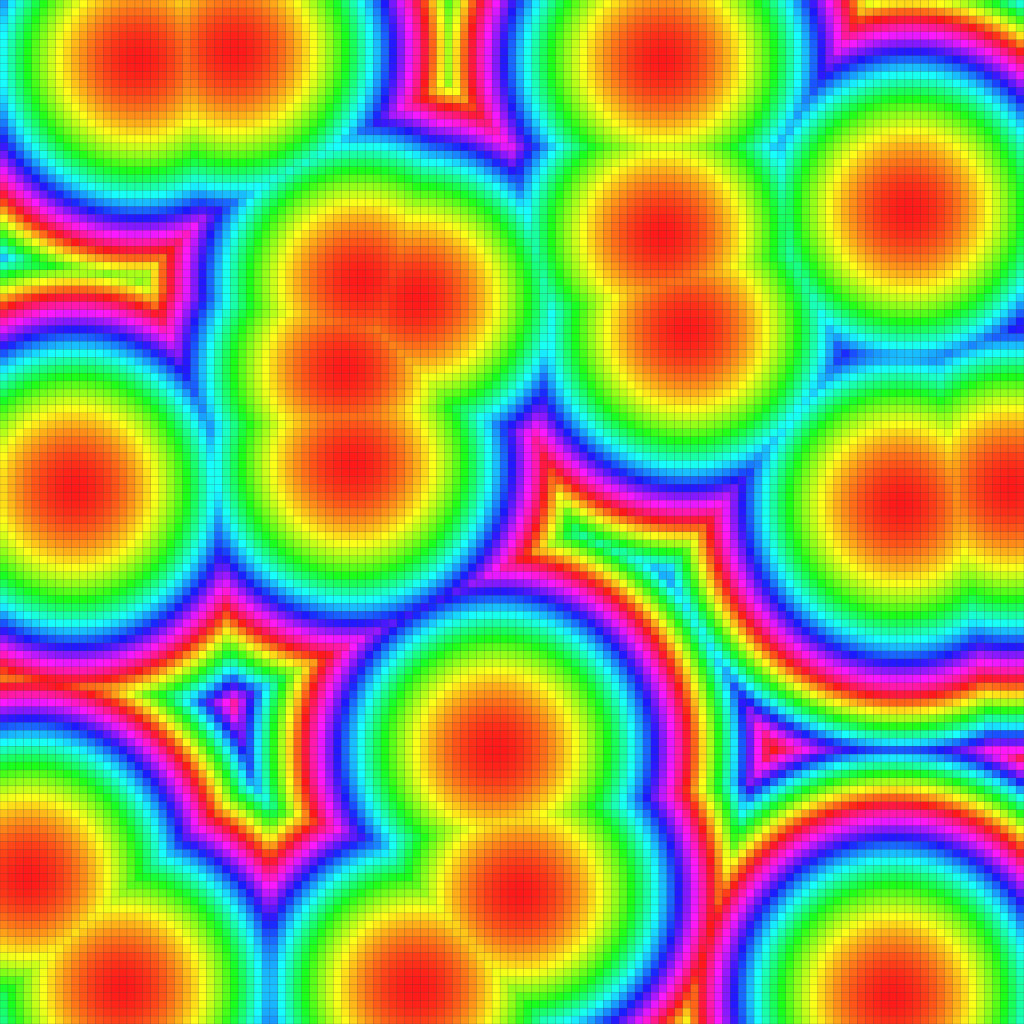
\includegraphics[width=3cm]{L2-2D}~~~~~
      
\includegraphics[width=3cm]{L1-2D}~~~~~
      
\includegraphics[width=3cm]{Linf-2D}\\
      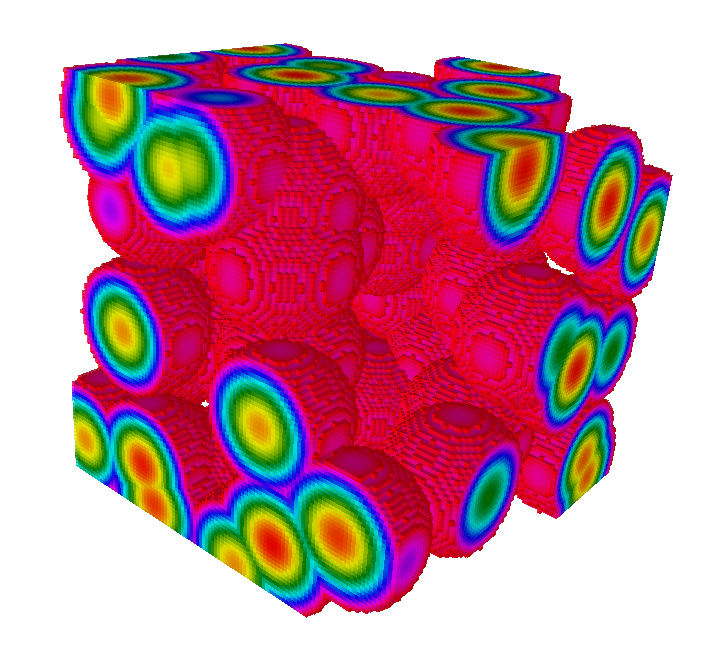
\includegraphics[width=3cm]{L2-3D}~~~~~
      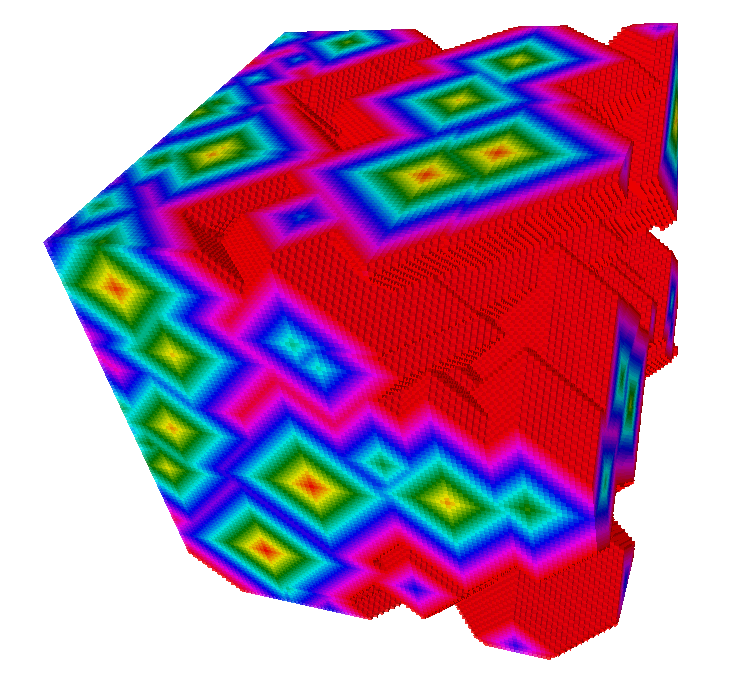
\includegraphics[width=3cm]{L1-3D}~~~~~
      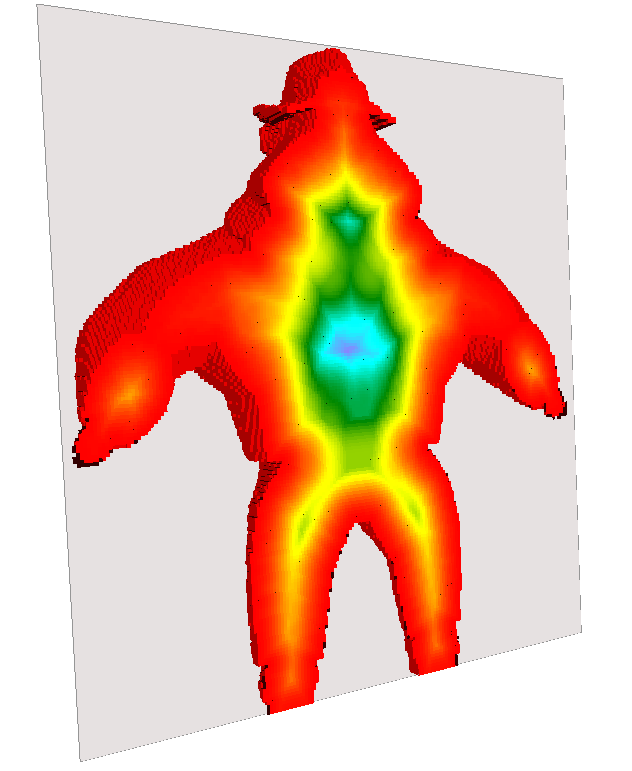
\includegraphics[width=3cm]{L2Al-3D}
    \end{center}
  \end{frame}

  \begin{frame}
    \frametitle{Future Works}

    \begin{exampleblock}{TODO list\HH}
      \begin{itemize}
      \item Voronoi/Power diagram mapping (OutputImage = ImageContainer<Point>)
      \item RMA extraction
      \item Benchmark/Improve memory managment
      \item Out-of-core versions (meta tiled image container?)
      \item Add tools (thickness diagram, MA simplification, \ldots)
      \item Volumetric based differential estimators
      \item QAT
      \end{itemize}
      
    \end{exampleblock}


    \begin{block}{Questions\HH}
      \begin{itemize}
      \item Mimic ITK/VTK image filters for volumetric transforms: e.g. output
        image as a DistanceTransformation class member and we return
        smart pointer ?
      \end{itemize}
    \end{block}

  \end{frame}
\end{document}



